\section{系统实现与应用验证}\label{sec:v2-application}

\subsection{架构与部署配置}

系统采用静态网页与 FastAPI 服务。用户从药物和溶剂目录中选择结构，输入温度并指定模型。服务将目录标识转换为完整 SMILES，核验模型文件的 SHA-256，加载相应预处理器与模型。默认模型版本为 \texttt{a3536da9c926}（文件散列前 12 位），使用全部开发记录拟合，树分支采用 869 维交互表示，预处理后输入 665 列，TabPFN 读取保存的训练上下文。系统按 ExtraTrees 权重 0.75、TabPFN 权重 0.25 计算对数溶解度，再按 CSV 的浓度字段对预测作 $10^{\widehat y}$ 反变换。图\ref{fig:v2-app-flow}给出服务处理链。

\begin{figure}[htbp]
\centering\small
\fbox{\begin{minipage}{0.91\linewidth}
\centering
分子目录与温度输入 $\longrightarrow$ 结构解析与描述符计算\\[4pt]
$\longrightarrow$ ExtraTrees 与 TabPFN 分支预测 $\longrightarrow$ 加权求和\\[4pt]
$\longrightarrow$ 预测值、分支输出与开发集数据覆盖
\end{minipage}}
\caption{默认模型从输入选择到结果展示的处理顺序。数据覆盖单独查询开发集，模型评价页另读取外层折外指标。}
\label{fig:v2-app-flow}
\end{figure}

\subsection{洛伐他汀在丙酮中的预测案例}

以洛伐他汀、丙酮和原始尺度温度 25 为例，界面返回对数溶解度 $-0.7270$，按 CSV 单位显示反变换浓度 $0.1875\,\mathrm{mol/L}$。ExtraTrees 预测约为 $-0.7221$，TabPFN 预测约为 $-0.7415$。用户可在同一药物和溶剂条件下查看温度曲线，或与基础 ExtraTrees 的预测作逐点比较。数据支持区域显示该组合有 20 条开发观测，温度覆盖为 5.5 至 49.5。这些观测构成部署模型的数据背景。系统另提供 CSV 批量入口用于比较候选条件。

\begin{figure}[H]
\centering
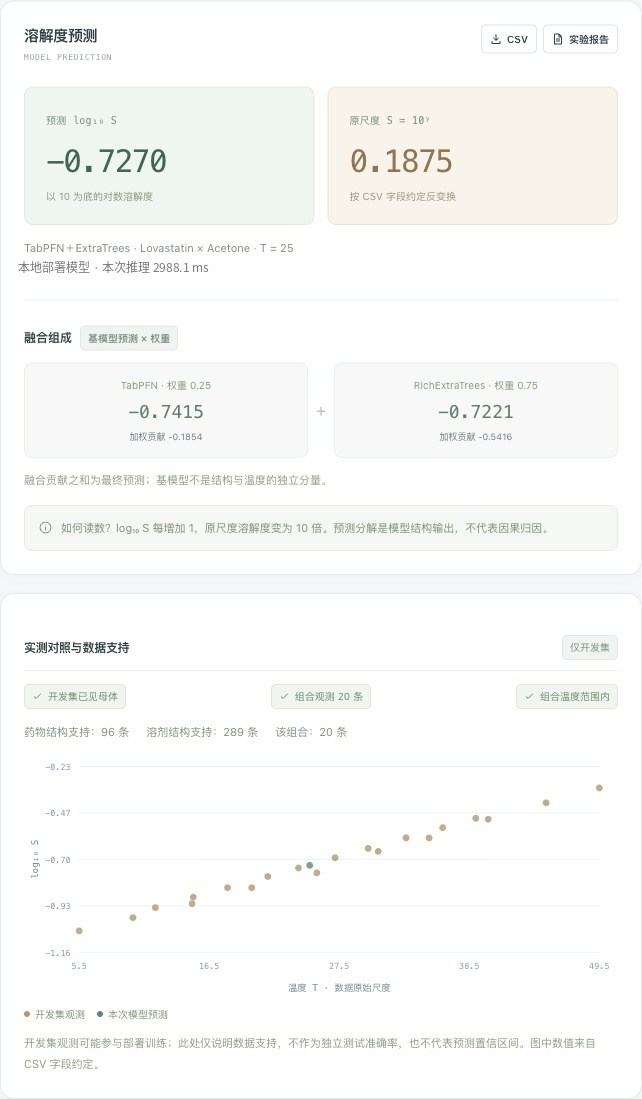
\includegraphics[width=\linewidth,height=0.51\textheight,keepaspectratio]{app_prediction.jpg}
\caption{应用中的洛伐他汀--丙酮单点预测。上部显示对数预测及反变换浓度，中部显示分支预测和权重，下部显示同一组合的开发集观测。温度采用 CSV 数值尺度。}
\label{fig:v2-app-example}
\end{figure}

\subsection{一致性、输入处理与运行表现}

通过进程内 HTTP 测试核对实际接口与离线模型。单点接口与离线调用在相同输入下达到 $10^{-8}$ 的对数预测绝对差容差，两个分支的加权贡献之和也与接口输出一致。对照接口对两个模型使用相同的 61 个温度点，并返回共同的 128 个母体的折外误差。该条件的 61 点曲线在温度 25 处与单点调用的绝对差为 $4.92\times10^{-7}$。批量接口允许 1--100 行，含无效温度的一行由该行返回错误，其余有效样本照常输出。复现脚本与核对结果保存在报告目录。
在 Apple Silicon 的 MPS 环境中，同一条件进行一次预热后，连续五次单行推理的服务端计时中位数为 2.32 秒，范围为 2.25 至 2.32 秒。该计时记录的是服务端模型计算，适用于此次设备和请求规模。
